\appendix

\chapter{Anhang}
\label{ch:Anhang}


%%%%%%%%%%%%%%%%%%%%%%%%%%%%
\section*{Gantt-Diagramm}
\label{app:Gantt-Diagramm}

\begin{center}
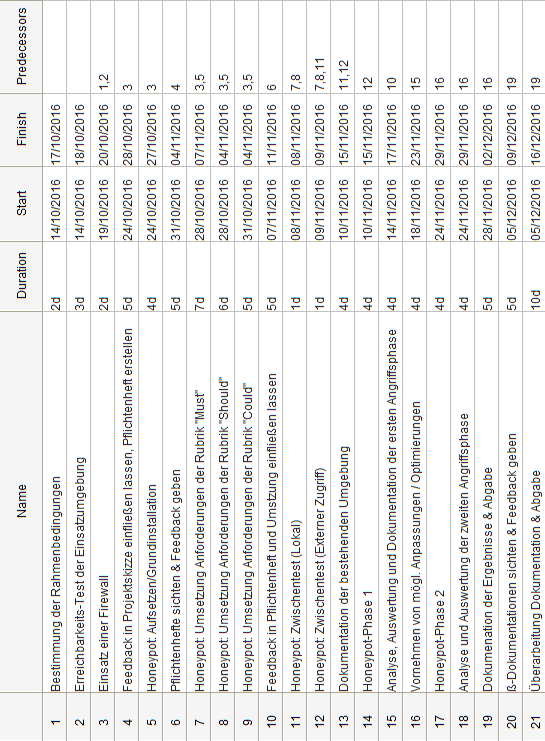
\includegraphics[scale=0.83]{img/gantt_tasks.png}
\end{center}

%%%%%%%%%%%%%%%%%%%%%%%%%%%%
\newpage

\begin{center}
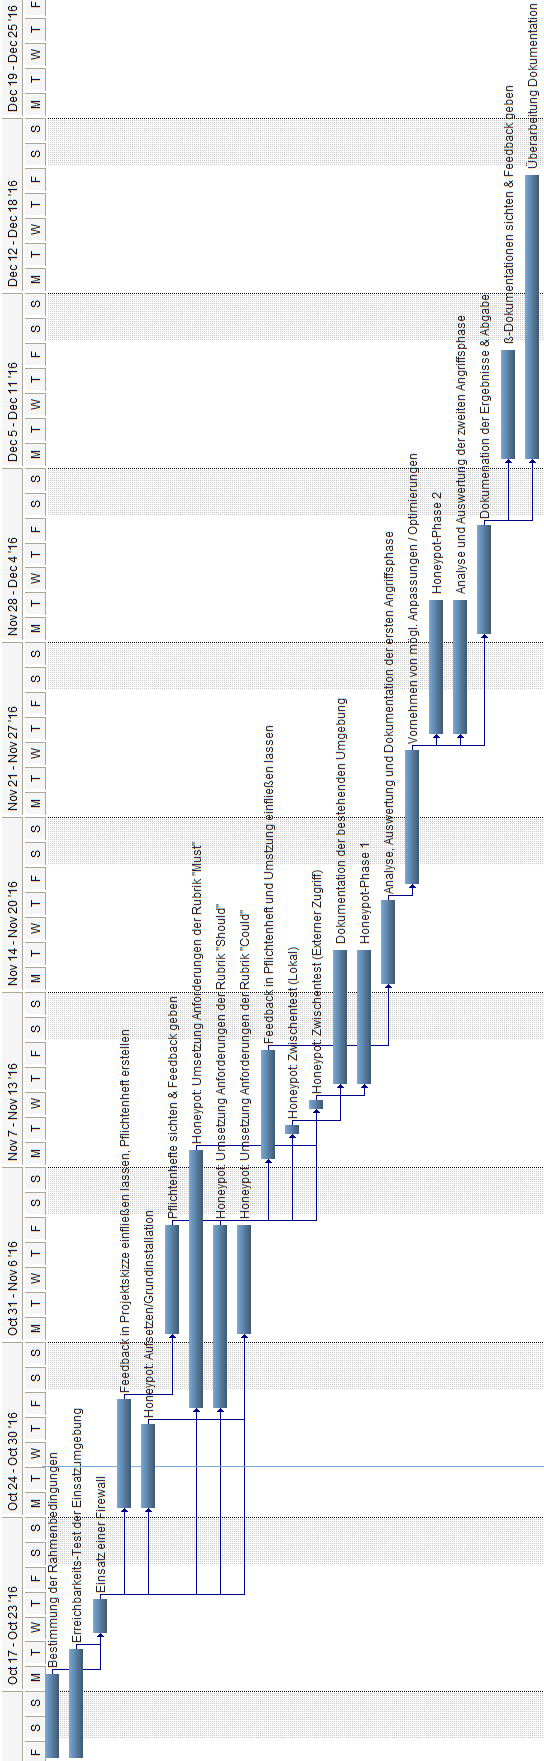
\includegraphics[scale=0.50]{img/gantt_diagram.png}
\end{center}

%%%%%%%%%%%%%%%%%%%%%%%%%%%%
\newpage

\section*{Ausschnitt aus Kippo-Logdatei}
\label{app:Ausschnitt aus Kippo-Logdatei}

%\lstinputlisting
%    [caption={Ausgabe der reverse-DNS-Auswertung}
%       \label{lst:reverse_dns},
%       captionpos=b,language={}]
% {listings/kippo_log.txt}

\begin{center}
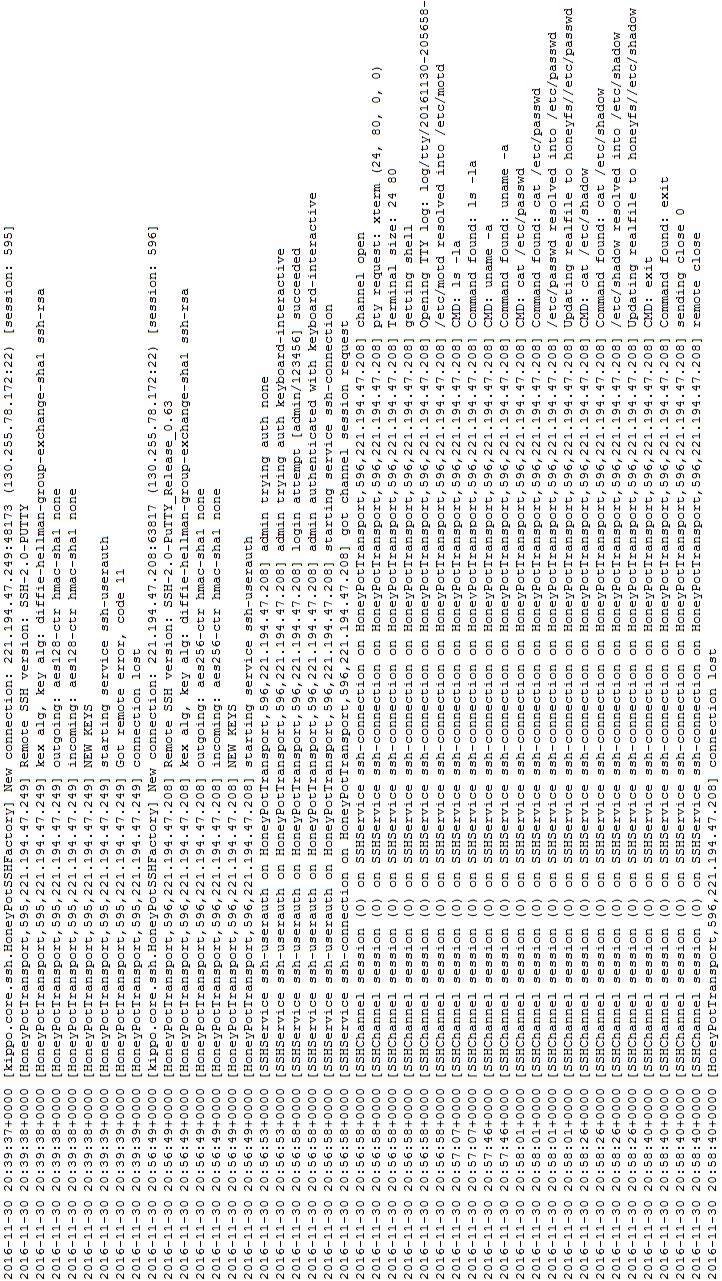
\includegraphics[scale=0.62]{img/kippo_log.png}
\end{center}


%%%%%%%%%%%%%%%%%%%%%%%%%%%%
\newpage

\section*{Benutzernamen und Passwörter extrahieren}
\label{app:Benutzernamen und Passwörter extrahieren}

\lstinputlisting
    [caption={Skript zur Extraktion von Benutzernamen und Passwörter aus Kippo-Logfile}
       \label{lst:mitm_onmsg},
       captionpos=b,language=bash,style=customccolor]
 {listings/extract_userdata.sh}
 
 
%%%%%%%%%%%%%%%%%%%%%%%%%%%% 
\newpage
 
\section*{Pipal Passwortstatistik}
\label{app:Pipal Passwortstatistik}

\lstinputlisting
    [caption={Passwortstatistik generiert durch Pipal Password Analzyer}
       \label{lst:mitm_onmsg},
       captionpos=b,language={}]
 {listings/pipal_statistik.txt}
 
 
%%%%%%%%%%%%%%%%%%%%%%%%%%%% 
\newpage 
 
\section*{Ausgabe iptables-save}
\label{app:Ausgabe iptables-save}

\lstinputlisting
    [caption={gekürzte Ausgabe von iptables-save}
       \label{lst:mitm_onmsg},
       captionpos=b,language={}]
 {listings/iptables-backup.txt}
 

%%%%%%%%%%%%%%%%%%%%%%%%%%%% 
\newpage 
 
\section*{Auswertung reverse-DNS-Lookup}
\label{app:Auswertung reverse-DNS-Lookup}

\lstinputlisting
    [caption={Ausgabe der reverse-DNS-Auswertung}
       \label{lst:reverse_dns},
       captionpos=b,language={}]
 {listings/reverse-dns.txt}
 
 
%%%%%%%%%%%%%%%%%%%%%%%%%%%% 
\newpage 
 
\section*{POST- und Path-Requests extrahieren}
\label{app:POST- und Path-Requests extrahieren}

\lstinputlisting
    [caption={Ausgabe der Path-Requests}
       \label{lst:snare-path-requests},
       captionpos=b,language={}]
 {listings/snare-path-requests.txt} 
 
 \lstinputlisting
    [caption={Ausgabe der POST-Requests}
       \label{lst:snare-post-requests},
       captionpos=b,language={}]
 {listings/snare-post-requests.txt} 
 